\documentclass[english]{beamer}
\usepackage[utf8]{inputenc}
\usepackage[T1]{fontenc}
\usepackage{amsfonts}
%\usepackage{amsthm}
\usepackage{makeidx}  % allows for indexgeneration
\usepackage{amsmath}
\usepackage{mathtools}
\usepackage{verbatim}
\usepackage{float}
\usepackage{graphicx}
\usepackage{times}  
%\usepackage[lined, boxed, linesnumbered]{algorithm2e}
\usepackage{array}
%\usepackage{makecell}
\usepackage{tikz}
\usepackage{lscape}
%\usepackage{caption}
%\usepackage{subcaption}
%\usepackage{subfig}

\beamertemplatenavigationsymbolsempty
\setbeamertemplate{footline}[frame number]

\usetheme{Antibes} % Beamer theme v 3.0
\usecolortheme{lily}

\title{A Column Generation Approach for the Virtual Network Embedding Problem}
\author{Leonardo F.S. Moura and Luciana S. Buriol}
\institute{Computer Science Department, Federal University of Rio Grande do Sul\\Porto Alegre, Brazil}
%\newtheorem{proposition}{Proposition}
%\newtheorem{theorem}{Theorem}[section]
%\newtheorem{lemma}{Lemma}[section]
\begin{document}
\begin{frame}
\titlepage
\begin{figure}
    \centering
    
\includegraphics[scale=0.4]{inf.png}
\end{figure}
\end{frame}

%---------------------------
\section{Introduction}
%---------------------------
\begin{frame}
\frametitle{Motivation}
Objective
\begin{itemize}
  \item Run one or more virtual networks on top of a physical network
\end{itemize}
Applications
\begin{itemize}
	\item Network Testbeds - New protocols can be tested without the need of 
      physical infrastructures.
	\item Geographical Network Presence - Companies can reduce the latency of
      communication with clients by renting physical structures.
	\item Cloud Computing - Client applications can share the same physical
      structure.
\end{itemize}
\end{frame}
%---------------------------
\begin{frame}
\frametitle{Virtual Network Embedding Problem}
\begin{columns}
\begin{column}{0.5\textwidth}
  \begin{figure}
    \centering
    \includegraphics[scale=0.4]{example.pdf}
  \end{figure}
\end{column}
\begin{column}{0.5\textwidth}
  \begin{figure}
    \centering
    \includegraphics[scale=0.32]{mapexample.pdf}
  \end{figure}
\end{column}
\end{columns}
	characteristics: one network at a time, Unsplittable paths, physical nodes host at most one virtual node
\end{frame}
%---------------------------
\begin{frame}
\frametitle{Research Questions}
\begin{itemize}
	\item Theoretically, how hard is the VNEP?
    \begin{itemize}
      \item NP-Complete
      \item (new result) Hard to approximate
    \end{itemize}
	\item In practice, what sizes of instances can be solved with exact methods?
    \begin{itemize}
      \item An integer solution to the problem is necessary.
      \item The problem of obtaining a feasible solution is hard (it is in NP-Complete).
      \item Online requests.
    \end{itemize}
\end{itemize}
\end{frame}
\begin{frame}
\frametitle{Exact Algorithms in The Literature}
\begin{itemize}
	\item Backtrack / Branch \& Bound \cite{Lischka2009} - Not exact
	\item ILP \cite{Chowdhury2010,Alkmim2013} - Lower quality relaxation
	\item Column Generation \cite{hu:2013} - No splittable paths in the literature
\end{itemize}
\end{frame}
%---------------------------
\begin{frame}
\frametitle{Solved as an Unsplittable Flow Problem}
\begin{columns}
\begin{column}{0.45\textwidth}
  \begin{figure}
    \centering
    \includegraphics[scale=0.4]{example.pdf}
  \end{figure}
\end{column}
\begin{column}{0.45\textwidth}
  \begin{figure}
    \centering
    \includegraphics[scale=0.4]{gaux.pdf}
  \end{figure}
\end{column}
\end{columns}
\end{frame}
%---------------------------
\begin{frame}
\frametitle{Relaxed ILP Model}
{\scriptsize
\begin{align}
  \min  & \sum\limits_{k \in E^{V}}\sum\limits_{p \in P^k}  c_{p} B_k z_{p} \nonumber \\
        & \sum\limits_{s \in V^{S}} x_{v,s} = 1                                  & \forall v \in V^{V} \label{eq:virone} \\
        & \sum\limits_{v \in V^{V}} x_{v,s} \leq 1                               & \forall s \in V^{S} \label{eq:subone} \\
        & \sum\limits_{p \in P^{k}} z_{p} = 1                                    & \forall k \in E^{V} \label{eq:virdemone} \\
        & \sum\limits_{k \in E^{V}}\sum\limits_{p \in P^{k}} \delta_{e,p} B_{k} z_{p} \leq B_{e} & \forall e \in E^{S} \label{eq:bandwidth} \\
        &  \sum\limits_{k \in E^{V}}\sum\limits_{p \in P^k : (v,s) \in p} z_{p} \leq M x_{v,s} & \forall v \in V^{V}, s \in V^{S} \label{eq:onlyoneaux}\\
        & 0 \leq x_{v,s} \leq 1  & \forall v \in V^{V}, s \in V^{S} \nonumber \\
        & 0 \leq z_{p}   \leq 1  & \forall p \in {P} \nonumber
\end{align}
}
\end{frame}
%---------------------------
\section{Column Generation Algorithm}
\begin{frame}
\frametitle{Column Generation Algorithm (Outline)}
\begin{enumerate}
	\item Find an initial set of columns
	\item Solve Restricted Master Problem
	\item Solve Auxiliary Problem
	\item If no new variables are found, terminate, otherwise add new variables and goto~2
\end{enumerate}
\end{frame}
%---------------------------
\begin{frame}
\frametitle{Auxiliary Graph Construction}
%\begin{align}
%  r_{p} = \sum\limits_{e \in p : e \in E^S} B_{k} (1 - y_{e}) - \sum\limits_{(v,s) \in p : (v,s) \notin E^S} \pi_{v,s} - \lambda_{k} \nonumber
%\end{align}

  \begin{figure}
    \centering
    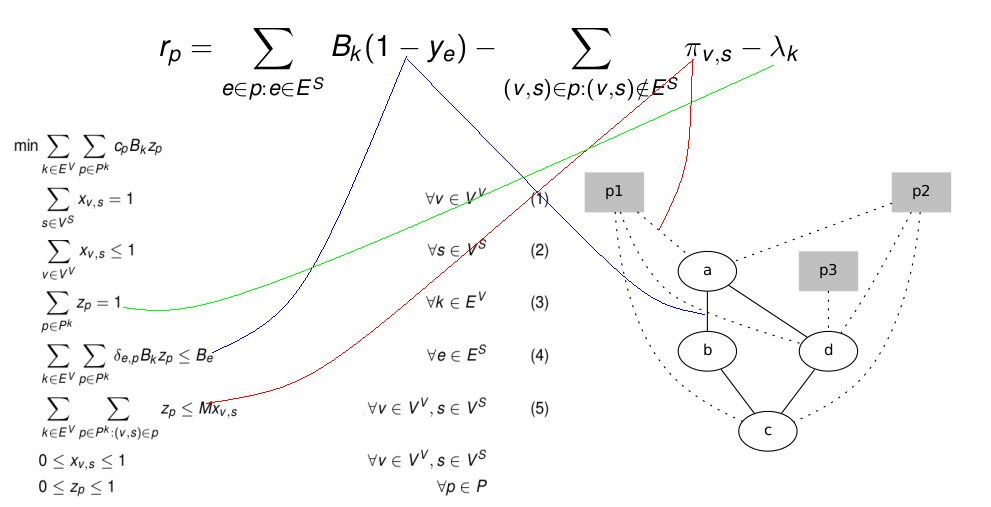
\includegraphics[scale=0.4]{redcost.png}
  \end{figure}

\end{frame}
%---------------------------
\section{Column Generation Algorithm}
\begin{frame}
\frametitle{Column Generation Algorithm}
\begin{enumerate}
	\item Find an initial set of columns
	\item Solve Restricted Master Problem
	\item Build auxiliary graph
	\item For each virtual link $k$
	\item \quad If there exists a path in the auxiliary graph with negative cost, add column to the model
	\item end if no paths were found in this iteration, otherwise goto~2
\end{enumerate}
\end{frame}
%---------------------------
\section{Results}

\begin{frame}
\frametitle{Experimental Approach}
All tests were performed on processor Intel Core i7 930 with 12~Gb of memory. 

The commercial solver CPLEX 12.5 was used to solve the relaxed and integer models. 

All instances were generated using the GTI-ITM tool
\end{frame}

\begin{frame}
\frametitle{Experimental Approach}
\begin{itemize}
  \item The CG algorithm bounds are compared with the optimal solution obtained with the ILP solved using CPLEX.

  \item Two sets of random instances were generated:
    \begin{itemize}
      \item Set1 - abundant resources
      \item Set2 - scarce resources
    \end{itemize}

  \item ``Since network virtualization is an emerging field, the actual characteristics of substrate networks and VN requests are still not well understood''
\cite{Chowdhury2010}

\end{itemize}
\end{frame}
%---------------------------
\begin{frame}
\begin{table}[h]
\begin{center}
\scriptsize
  \begin{tabular}{c c | r r r | r r}
$|S|$ & $|V$| &  \#unf & \#limit &  GAP\%   &  CG(s)        &  CPLEX(s)    \\
\hline
10 & 2     & 0 & 0 &   0.00     &  0.01$\pm$0.00   &  0.01$\pm$0.00(9)        \\
20 & 2     & 0 & 0 &   0.00     &  0.01$\pm$0.00   &  0.02$\pm$0.00(9)        \\
40 & 2     & 0 & 0 &   0.00     &  0.01$\pm$0.00   &  0.04$\pm$0.01(9)        \\
80 & 2     & 0 & 0 &   0.00     &  0.01$\pm$0.00   &  0.21$\pm$0.05(9)        \\
10 & 4     & 2 & 0 &   10.20    &  0.01$\pm$0.00   &  0.05$\pm$0.03(9)        \\
20 & 4     & 0 & 0 &   6.77     &  0.01$\pm$0.00   &  0.12$\pm$0.05(9)        \\
40 & 4     & 0 & 0 &  0.00     &  0.01$\pm$0.00   &  0.37$\pm$0.17(9)        \\
80 & 4     & 0 & 0 &   0.00     &  0.01$\pm$0.00   &  3.17$\pm$0.92(9)        \\
20 & 8     & 5 & 0 &   0.10     &  0.01$\pm$0.00   &  0.92$\pm$0.88(9)        \\
40 & 8     & 0 & 0 &   4.48     &  0.01$\pm$0.00   &  10.84$\pm$10.32(9)      \\
80 & 8     & 0 & 8 &   0.00     &  0.01$\pm$0.00   &  887.92$\pm$43.36(9)     \\
40 & 16   & 0 & 0 &   20.19    &  0.02$\pm$0.00   &  594.58$\pm$86.23(9)    \\
\hline                                                                                          
10 & 2    & 6 & 0 &   0.00      &  0.00$\pm$0.00 &  0.01$\pm$0.00        \\
20 & 2    & 4 & 0 &   0.00      &  0.00$\pm$0.00 &  0.02$\pm$0.00        \\
40 & 2    & 3 & 0 &   0.00      &  0.00$\pm$0.00 &  0.03$\pm$0.00        \\
80 & 2    & 4 & 0 &   0.00      &  0.01$\pm$0.00 &  0.18$\pm$0.04        \\
20 & 4    & 6 & 0 &   7.23      &  0.00$\pm$0.00 &  0.08$\pm$0.06        \\
40 & 4   & 4 & 0  &  0.00      &  0.00$\pm$0.00 &  0.26$\pm$0.23         \\
80 & 4    & 2 & 0 &   5.79      &  0.01$\pm$0.00 &  2.56$\pm$2.48        \\
40 & 8    & 8 & 0 &  5.68       &  0.00$\pm$0.00 &  0.96$\pm$0.34        \\
80 & 8    & 5 & 0 &  16.24      &  0.01$\pm$0.01 &  10.32$\pm$10.42    \\
\end{tabular}
\end{center}
\end{table}
\end{frame}
%---------------------------
\section{Conclusion}
\begin{frame}
\frametitle{Conclusions}
Contribution
\begin{itemize}
	\item New CG model for unsplittable flow
	\item A good quality lower bound is obtained in a timely fashion.
\end{itemize}

Future Works
\begin{itemize}
	\item Search for Lower Bounds.
	\item This work is being extended to a Branch \& Price algorithm.
	\item A further study on the Virtual Network Embedding Problem.
\end{itemize}
\end{frame}
%---------------------------
\begin{frame}
\frametitle{Planejamento}
\begin{itemize}
	\item Maio: submissão para SBPO em conjunto com bolsista
	\item Maio: submissão de artigo para ALIO/EURO 2014
	\item Junho-Setembro: escrita da dissertação
	\item Julho: submissão para revista
  \item Setembro/Outubro: apresentação dissertação
\end{itemize}
\end{frame}

\begin{frame}
\bibliographystyle{splncs}
\bibliography{VNE}
\end{frame}
\end{document}



%---------------------------
\begin{frame}
\frametitle{teste}

\end{frame}








\pagestyle{headings}

\maketitle


\section{Introduction}
Network virtualization was proposed for overcoming the problem of ossification of the Internet, a way to facilitate the evolution of the protocols of the Internet.
%~\cite{Anderson2005}. 
In virtualized environments, multiple networks can simultaneously use the same physical structure in a transparent way. By creating a new layer of abstraction over the physical networks, new protocols can be tested on heterogeneous experimental architectures~\cite{Anderson06geni}. Likewise, service providers can offer customized services, like customized protocols, or co-location for expanded network presence, by leasing resources from infrastructures providers (InPs)~\cite{Feamster:2007}. Virtualization is being used in practice~\cite{Carapinha:2009,Anderson06geni} and it is considered the main enabling technology for cloud computing.

The Virtual Network Embedding Problem (VNEP) is central to achieve network virtualization. 
It consists in mapping multiple virtual networks with heterogeneous architectures on a single substrate physical network.
Virtual nodes are mapped to physical substrate nodes which are interconnected by a path in the physical substrate corresponding to the mapping of virtual links. 
Additionally, the physical resources have limitations that need to be taken into account by the mapping. 
The main objective of the VNEP is to minimize the use of the underlying resources such as bandwidth, while attending the mapping constraints.

There are several variations of the problem such as mapping several networks simultaneously~\cite{Yu2008,Chowdhury:2012,Alkmim2013}, instead of a single one at a time~\cite{hu:2013}.
Moreover, networks can also be mapped in an online fashion, lasting for a period of time, using and releasing physical resources dynamically~\cite{Yu2008}. 
Physical nodes and links can be restricted to host a limited number of virtual nodes and links.
Depending on the context of the problem, security restrictions are also required, limiting the subset of physical nodes and links that can be used for mapping~\cite{Buriol:2012}.
  Finally, paths can be splittable~\cite{Yu2008,Chowdhury:2012,hu:2013} or not~\cite{Alkmim2013}.
If splittable flow is allowed, each virtual link can be mapped to more than one path in the physical substrate, 
such that its demand of bandwidth is attended.
By allowing path splitting, simpler algorithms can be used for virtual link mapping. 
Path splitting however is not always feasible, can incur in extra costs for InPs, and can violate security constraints.
Surveys of the different models and constraints can be found in~\cite{Chowdhury2010,FischerSurvey}.

The VNEP is NP-Hard \cite{Lischka2009} % and there is no efficient algorithm that finds a feasible solution for the problem (the proof is presented in Section~\ref{sec:complexity}). 
and it can be modeled as an Integer Linear Programming (ILP) problem. 
Flow-based ILP models are presented in the literature. 
A model with splittable paths is presented in~\cite{Chowdhury:2012}, while with unsplittable paths is presented in~\cite{Alkmim2013}. 
Both works present a rounding scheme to obtain integer solutions from the relaxation of the integer models.
However, heuristic methods or rounding schemes do not guarantee to find a feasible solution. 
On the experimental side, only small instances are solved up to optimality with a general purpose solver within a reasonable amount of time.
A natural attempt in solving this problem efficiently is by using problem specific exact algorithms, instead of general purpose solvers.
Developing specialized cuts for integer models or devising better bounds on the optimal solution are important ingredients
to improve exact algorithms. 


For minimization problems, the relaxation of integer linear programming (ILP) models yields lower bounds on the value of the optimal solution of the original problem. 
Obtaining high quality bounds on the optimal integer solution can greatly reduce the running time of exact algorithms. 
However, the relaxation of a classic ILP model of this problem results in trivial lower bounds.

%In \cite{hu:2013}, a path-based model with path splitting is presented. 


In this work we propose a column generation approach, based on a path-based model, to generate bounds for the VNEP. 
We adapted the path-based model and column generation approach for path splitting proposed by~\cite{hu:2013} for the case of unsplittable paths.
Since the number of paths in graphs grows exponentially with the size of the graph, a column generation algorithm is applied with the aim of generating a high quality lower bound for the problem. 
%The linear relaxation of that model results in a high quality lower bound than the linear relaxation of the flow formulation.
We consider the case of mapping a single virtual network, and each physical node is restricted to host a single virtual link.
The paper is structured as follows: In Section~\ref{sec:problem}, the Virtual Network Embedding Problem is formalized while in Section~\ref{sec:CG} the column generation algorithm is presented. 
Section~\ref{sec:results} presents experimental results and their analysis. Finally, Section~\ref{sec:conclusion} concludes this work, presenting suggestions for future lines of research.



\section{Virtual Network Embedding Problem}
\label{sec:problem}

The VNE problem takes as input a physical and a virtual networks.
The physical substrate network is modelled as an undirected graph $N^{S}=(V^{S},E^{S})$. Each node $v \in V^{S}$ represents a substrate node with a CPU capacity of $C_{v}$. Each edge $e \in E^{S}$ represents a physical link with bandwidth capacity $B_{e}$. Similarly, the virtual network is modelled as a directed graph $N^{V}=(V^{V},E^{V})$. Each node $v \in V^{V}$ represents a virtual node with a CPU demand of $C_{v}$. Each arc $e \in E^{V}$ represents a virtual link with bandwidth demand~$B_{e}$.

The goal of the problem is to find a mapping $f1: V^V \rightarrow V^S$ of the nodes and a 
mapping $f2: (u,v) \in V^V \rightarrow u'\leadsto v'$ of the links, where $u' \leadsto v'$ stands for a path between nodes $u',v' \in V^S$. 
Each substrate node can host at most one virtual node, attending the residual capacity restriction. 
Each virtual link $(u,v)$ has to be mapped to a $u'\leadsto v'$-path in the substrate graph, if $u \in V^V$ is mapped to $u'\in V^S$ and $v\in V^V$ to $v' \in V^S$. 
The amount of bandwidth required by the hosted virtual links cannot exceed the capacity of the substrate link.
By mapping a single network, the amount of CPU resources used by the virtual network is the same for each feasible mapping. 
Thus the objective function is to minimize the amount of bandwidth used for the mapping. %This means that the smaller the paths used, the better.

Figure~\ref{fig:example}-left presents an instance of the problem composed of a physical network with four nodes and a virtual network with three nodes. Next to the edges are their capacities or demands. Next to each node label is the capacity or demand of the node.
The optimal mapping is shown in Figure~\ref{fig:example}-right. 
%Since the substrate node $d$ is the only one with enough capacity to host $p3$, 
An optimal solution is to map $p1$ to $c$, $p2$ to $a$, and $p3$ to $d$;
the virtual link $(p2,p3)$ is mapped to $a-d$ and $(p1,p2)$ to $a-d-c$. The cost of this solution is $50$.

\begin{figure}
  \centering
  \begin{subfigure}[b]{0.45\textwidth}
    \centering
    \includegraphics[scale=0.4]{example.pdf}
%    \caption{A VNEP instance.\label{fig:auxcex}}
  \end{subfigure}\quad
  \begin{subfigure}[b]{0.45\textwidth}
    \centering
    \includegraphics[scale=0.3]{mapexample.pdf}
%    \caption{Optimal mapping\label{fig:mapping}.}
  \end{subfigure}
  \caption{A VNEP instance composed by a physical substrate and a virtual network (left) and the corresponding optimal mapping (right).
In the figure on the right, solid lines represent original links, dashed lines represent the node mapping, while dotted lines corresponds the link mapping.
\label{fig:example}}
\end{figure}

%\subsection{Complexity}
%\label{sec:complexity}
%There is no efficient algorithm that finds an approximate solution for the VNEP with unsplittable paths, unless $P=NP$.

%proof \ldots




\subsection{A Compact ILP Model}
\label{sec:ILPmodel}
The following model is based on \cite{Alkmim2013}. Since the aim of this work is to generate high quality lower bounds to be used in exact algorithms, we basically consider a simplified version of the problem from~\cite{Alkmim2013} by removing some constraints.
Let the decision variables~$x_{v,s} = 1$ iff the substrate node $s$ hosts the virtual node $v$. And let $\Delta_{v,w,s,j} = 1$ iff the physical link $(s,j)$ hosts the virtual link $(v,w)$.

%\scriptsize

\begin{align}
    \min & \sum\limits_{(s,j) \in E^{S}} \sum\limits_{(v,w) \in E^{V}} \Delta_{v,w,s,j} B_{v,w} \nonumber \\
    s.t. & \sum\limits_{v \in V^{V}} x_{v,s} C_{v} \leq C_{s}                     & \forall s \in V^{S}  \label{eq:flowcap} \\
    & \sum\limits_{s \in V^{S}} x_{v,s} = 1                                  & \forall v \in V^{V}  \label{eq:flowvirone}\\
         & \sum\limits_{v \in V^{V}} x_{v,s} \leq 1                               & \forall s \in V^{S} \label{eq:flowsubone}\\
         & \sum\limits_{j \in V^{S}} \Delta_{v,w,s,j} - \sum\limits_{j \in V^{S}} \Delta_{v,w,j,s} = x_{v,s} - x_{w,s}  & \forall (v,w) \in E^{V}, s \in V^{S}\label{eq:flowflow} \\
         & \sum\limits_{(v,w) \in E^{V}} \Delta_{v,w,s,j} B_{v,w} \leq B_{s,j}  & \forall (s,j) \in E^{S} \label{eq:flowbandwidth} \\
         & x_{v,s} \in \{0,1\} & \forall v \in V^{V}, s \in V^{S} \\
         & \Delta_{k,l,m,n} \in \{0,1\} & \forall (k,l) \in E^{V}, (m,n) \in E^{S}
\end{align} 

The objective function minimizes the amount of bandwidth used. 
Constraints~\eqref{eq:flowcap} ensure that the substrate capacities are not surpassed. 
Constraints~\eqref{eq:flowvirone} enforce that every virtual node is mapped to a substrate node, while~\eqref{eq:flowsubone} enforce that every substrate node hosts at most one virtual node. 
Constraints~\eqref{eq:flowflow}
ensure that every virtual link is mapped to a path into the substrate graph. Finally, constraints~\eqref{eq:flowbandwidth} ensures that the bandwidth capacities of the physical edges are not violated.

A relaxation of this model naturally results in no mapping, since Equation~\eqref{eq:flowflow} does not enforce the mapping of virtual links. 
In the optimal solution of the relaxation $x_{vs}-x_{ws}=0$ in Eq.~\ref{eq:flowflow}  and then
all variables $\Delta_{v,w,s,j}$ are set to~$0$ . 
Therefore, the value of the optimal solution for the relaxed problem is always $0$, resulting in a trivial lower bound.




\subsection{A Path-Based ILP Model}
Traditionally, the virtual network embedding is executed in two steps: the node mapping, and then the link mapping. 
The following approach, based in~\cite{Chowdhury:2012}, uses an auxiliary graph $H$ to execute both mappings in a single phase. 
Graph $H$ is basically the substrate graph added of~$|V^{V}|$ meta nodes, one for each virtual node. 
Those meta nodes are linked by meta edges to all substrate nodes that have enough capacity to host them. 
%Thus, each virtual link can be viewed as a commodity with terminals in its endpoints. 
The problem of mapping edges and nodes of the original problem is reduced to a modified unsplittable flow problem. 
This new problem consists in finding a set of paths that covers all virtual links without violating the capacity constraints. 
Also, each virtual link uses exactly two meta edges, which guarantees that a valid set of paths yield a valid solution for the VNEP.
%If a meta edge $(v,s)$ is used, then the virtual node $v$ is mapped to the substrate node $s$. 
So, for example, if two virtual nodes $u$ and $v$ are linked by a path in the auxiliary graph containing the meta edges $(u,s)$ and $(t,v)$, that means that $u$ is mapped to $s$, and $v$ is mapped to $t$.
%Traditionally, the virtual network embedding is executed in two steps: The node mapping, and the link mapping. 
%In this formulation, an auxiliary graph is used so that the mappings are executed in a single phase. 
%On the top of the substrate graph are added~$|V^{V}|$ meta nodes, one for each virtual node. 
%Those meta nodes are linked to all substrate nodes that have enough capacity to host them. 
%Thus, if two virtual nodes $u$ and $v$ are linked by a path in the substrate graph containing the meta edges $(u,s)$ and $(t,v)$, that means that $u$ is mapped to $s$, and $v$ is mapped to $t$.
%An example auxiliary graph is shown in Figure~\ref{fig:aux}. 

Figure~\ref{fig:aux} shows an example of the auxiliary graph for Figure~\ref{fig:example}.
Meta nodes $p1$, $p2$, and $p3$ are added on top of the substrate graph. If the virtual link $(p2, p3)$ is mapped to the path $p2-a-d-p3$, the node $p2$ is mapped to $a$, and $p3$ to $d$.

\begin{figure}[h!]
  \centering
  \includegraphics[scale=0.3]{gaux.pdf}
  \caption{Auxiliary graph for the example from Figure~\ref{fig:example}.\label{fig:aux}}
\end{figure}

The following formulation is adapted from \cite{hu:2013} to accommodate unsplittable paths. 
Two set of decision variables are used: For each $v \in V^{V}$ and $s \in V^{S}$, the variable $x_{v,s} \in \{0,1\}$ is set to one iff the substrate node $s$ hosts the virtual node $v$. 
Likewise, for each path $p$ in the set of all paths $P$, the variable $z_{p} \in \{0,1\}$ is set to one if the path is used in the VNE. 
Each virtual link $k=(v,w) \in V^V$ has a set $P^k$ of all simple paths linking the endpoints nodes of $k$ to the nodes they were mapped in the substrate graph.

\begin{align}
  \min  & \sum\limits_{k \in E^{V}}\sum\limits_{p \in P^k}  c_{p} B_k z_{p} \label{eq:obj} \\
        & \sum\limits_{s \in V^{S}} x_{v,s} = 1                                  & \forall v \in V^{V} \label{eq:virone} \\
        & \sum\limits_{v \in V^{V}} x_{v,s} \leq 1                               & \forall s \in V^{S} \label{eq:subone} \\
        & \sum\limits_{p \in P^{k}} z_{p} = 1                                    & \forall k \in E^{V} \label{eq:virdemone} \\
        & \sum\limits_{k \in E^{V}}\sum\limits_{p \in P^{k}} \delta_{e,p} B_{k} z_{p} \leq B_{e} & \forall e \in E^{S} \label{eq:bandwidth} \\
        &  \sum\limits_{k \in E^{V}}\sum\limits_{p \in P^k : (v,s) \in p} z_{p} \leq M x_{v,s} & \forall k \in E^{V}, \forall v \in V^{V}, s \in V^{S} \label{eq:onlyoneaux}\\
        &  x_{v,s} \in \{0,1\}  & \forall v \in V^{V}, s \in V^{S} \nonumber \\
        & z_{p} \in \{0,1\}    & \forall p \in {P} \nonumber
\end{align}

The objective function is the minimization of the total bandwidth used by the virtual network. If a path $p$ serves a virtual link $k$, the cost of this path $c_{p}$ is defined as the number of physical edges in this path.
Equation~\eqref{eq:virone} ensures that all virtual nodes are mapped. Each substrate node can host at most one virtual node~\eqref{eq:subone}.
Equation~\eqref{eq:virdemone} states that all virtual links have to be mapped to a single path in the substrate graph. Equation~\eqref{eq:bandwidth} ensures that the bandwidth constraints are not violated.
Equation~\ref{eq:bandwidth} requires the input data $\delta_{e,p}$ which is set to one iff the substrate link $e$ is used by the path $p$.
Finally, Equation~\eqref{eq:onlyoneaux} enforces that only valid meta edges are used, where M is a large number.
%. Let M be a large number, and $P^{k}$ be the set of all paths that cover the virtual link $k$. Suppose that a certain variable $x_{v,s}$ is set to one. Only the paths that pass through the meta edge $(v,s)$ can be used.



\section{Column Generation for the VNEP}
\label{sec:CG}

Since the resolution of the integer VNEP is computationally expensive, 
this work focus on solving the relaxation of the path-based ILP model presented in the previous section by using a column generation (CG) algorithm.
Column generation is a mathematical programming technique proposed by Dantzig and Wolfe \cite{Dantzig:1960} 
to solve models with a large number of variables.
These ``large'' models usually provide better bounds on the optimal integer solutions than compact models, and this is the case for the VNEP.
The restricted master problem, comprised of a subset of variables (columns), is solved at each iteration of the CG.
At each iteration, new columns are generated implicitly and added to the restricted master problem.
Columns are obtained solving a pricing problem.
The pricing problem, in a minimization problem, finds the column with the minimum reduced cost.
If the minimum reduced cost is positive, the restricted master problem is optimal.

Let $\lambda$, $y$, and  $\pi$ be the dual variables related to the constraints \eqref{eq:virdemone}, \eqref{eq:bandwidth}, and \eqref{eq:onlyoneaux}, respectively. The reduced cost of each variable $z_{p}$ that covers the virtual link $k$ is:

\begin{align}
  c_{p} B_{k} - \lambda_{k} + \sum\limits_{e \in p : e \in E^S} B_{k} y_{e}  + \sum\limits_{(v,s) \in p : (v,s) \notin E^S} \pi_{v,s}  \nonumber
\end{align}

Since $c_p$ is the number of edges on the path $p$, the equation above is equivalent to:

\begin{align}
  \sum\limits_{e \in p : e \in E^S} B_{k} (y_{e} + 1) + \sum\limits_{(v,s) \in p : (v,s) \notin E^S} \pi_{v,s} - \lambda_{k} \nonumber
\end{align}

Thus, the minimum reduced cost for the VNEP is obtained by solving the following problem:

\begin{align}
  \min_{ \forall k \in E^{V}, \forall p \in P^{k}}  \quad  \sum\limits_{e \in p : e \in E^S} B_{k} (y_{e} + 1) + \sum\limits_{(v,s) \in p : (v,s) \notin E^S} \pi_{v,s}-\lambda_{k} \nonumber
\end{align}

Each column in the model corresponds to a path in the auxiliary graph. At each iteration, for each virtual link $k = (v,w) \in E^V$, a shortest path is calculated in the auxiliary graph. A path is composed of two auxiliary edges and a set of edges from the substrate graph. To minimize the function above is equivalent to find a path in the modified auxiliary graph where the meta edges $(v,s)$ have a cost of $\pi_{v,s}$ and the substrate edges $e$ have a cost of $B_{k}(y_{e} + 1)$. If a shortest path with a negative value is obtained, the generated column is added to the restricted master problem. Otherwise, the current set of columns provides the optimal solution for the master problem.

%As the number of possible paths grows exponentially with the size of the substrate graph, a column generation algorithm is used. 
%This problem uses a limited set of variables, or columns, related to an initial set of paths $P' \subseteq P$. 
%If no path $p$ exists that respect this constraint, that dual problem is unfeasible and the solution of the restricted master problem is equal to the problem with all paths. Therefore the optimal solution is obtained.\\
%The auxiliary graph is set in such a way that to search a path in it that serves $k$ with cost smaller than $\lambda_{k}$ is tantamount to find a new column for the primal problem. Therefore a proof of optimality for the selected set of paths in the restricted master problem is given if no such paths exist in the auxiliary graph.

Algorithm~\ref{alg:cg} summarizes the column generation algorithm. In~Line~\ref{alg:genpath} the initial set of columns is generated, as described in Section~\ref{sec:initialCol}. With these initial set of paths, the restricted master problem is solved in Line~\ref{alg:solve}. From the solved restricted master problem, the dual variables are obtained and the auxiliary graph is constructed in Line~\ref{alg:buildaux}. For each virtual link~$(v,w)$ in the virtual network, a path $p$ is calculated in the auxiliary graph in Line~\ref{alg:findpaths}. If $p$ costs less than $\lambda_{k}$, the dual variable related to Constraints~\eqref{eq:virdemone}, then $p$ is added to the set of all paths. The restricted master problem, including $p$, is again solved and the procedure is repeated until no paths are added in a given iteration. 
Finally, if some variable~$v_{e}$ is greater than zero, than the original problem is unfeasible, and this is tested in Line~\ref{alg:feascond}.
\begin{algorithm}
%\SetKwInOut{Input}{input }
%\Input{j : first item, z : profit, c : capacity}
%\scriptsize
find initial set of paths\; \label{alg:genpath}
\Repeat{No paths were added to $P'$}
  {solve model with limited set of columns $P'$\; \label{alg:solve}
  obtain dual variables $\lambda$, $y$, and $\pi$\; 
  update weights of the edges of auxiliary graph $H$\; \label{alg:buildaux}
  \For{virtual link $k \in E^{V}$}
    {find min path $p$ in $H$ with cost $c_{p}$\; \label{alg:findpaths}
    \If{$c_{p} \leq \lambda_{k}$}
      {add paths to $P'$\;}
    }
  }
\eIf{$\forall e \in E^{S} (v_{e} = 0)$ \label{alg:feascond}}
  {the problem is solved optimally\;}
  {the problem is unfeasible\;}
\caption{Column Generation Algorithm for VNE}
\label{alg:cg}
\end{algorithm}

\subsection{Generation of the initial paths}\label{sec:initialCol}
To satisfy Equation~\ref{eq:virdemone}, the initial set of paths $P'$ has to contain at least one feasible path for each virtual link.
%The initial set of columns are found heuristically. 
%We then designed the following algorithm.
Initially the virtual nodes are ordered decreasingly according to their demands. The same is done for the substrate nodes, considering their resources.
According to this order, each virtual node is mapped to the first free physical node that has enough resources to host it.
When both nodes of a virtual link are mapped, the path with minimum hop count is then calculated between the corresponding physical nodes.
If no path exists, any other path that can host the virtual nodes and links is then considered.
When mapping a node, if there is no free physical node, then the virtual node is mapped to the first non-free physical node that has enough resources to host it.
In case there is not such a node, the algorithm stops since there is no possible mapping for the instance.

%Having the nodes mapped, the least cost path
%A path of minimum number of hops on the substrate graph is then calculated to each virtual links, considering the nodes to where its endpoints were mapped.
%The pairs of nodes are matched in order and a path is searched for in the substrate graph. 
%If no valid path is found, then any path whose endpoints have enough capacity to hold the endpoints of the virtual node is searched. 
%If no such pair is found, the problem is infeasible and the whole algorithm stops.

%colei a parte abaixo de cima...
For the column generation algorithm to work properly, the initial set of columns has to yield a feasible solution. 
%Since finding a feasible solution for the problem {\color{red} is computationally intractable}, 
For that, a variable $v_{e}$ is added to each capacity constraint in~\eqref{eq:bandwidth}. 
Each $v_{e}$ represents the amount of bandwidth violation in the substrate edges. 
A penalty $K$ is added to the objective function for each violation. 
The penalty value $K$ is set to be the sum of all demands of the virtual link, so that any feasible solution has a smaller objective value than any solution that violates a bandwidth constraint.

\iffalse
\begin{align}
    \min & \sum\limits_{p \in P}  z_{p} c_{p} + \sum\limits_{e \in E^{S}} K v_{e} \nonumber \\
    s.t. & \sum\limits_{s \in V^{S}} x_{v,s} = 1                                  & \forall v \in V^{V} \label{eq:virone2} \\
         & \sum\limits_{v \in V^{V}} x_{v,s} \leq 1                               & \forall s \in V^{S} \label{eq:subone2}\\
         & \sum\limits_{p \in P^{k}} z_{p} = 1                                    & \forall k \in E^{V} \label{eq:virdemone2}\\
         & \sum\limits_{k \in E^{V}}\sum\limits_{p \in P^{k}} \delta_{e,p} B_{k} z_{p} \leq B_{e} + v_{e}               & \forall e \in E^{S} \label{eq:bandwidth2} \\
         & \sum\limits_{p \in P : (v,s) \in p}  z_{p} \leq M x_{v,s} & \forall v \in V^{V}, \forall w \in V^{V}, s \in V^{S} \label{eq:onlyoneaux2} \\
         & 0 \leq x_{v,s} \leq 1  & \forall v \in V^{V}, s \in V^{S} \nonumber \\
         & 0 \leq z_{p} \leq 1    & \forall p \in {P} \nonumber \\
         & 0 \leq v_{e}           & \forall e \in E^{S} \nonumber
\end{align} 
\fi



\subsection{Update of the auxiliary graph weights}\label{sec:update}
In Line~\ref{alg:buildaux} of the Algorithm~\ref{alg:cg} the weights of the auxiliary graph are updated.
To each auxiliary edge $(v,s)$ is assigned a cost of $\pi_{v,s}$. 
To each substrate edge $e$ is assigned a cost of $B_{k}(y_{k} + 1)$. 
Thus, the cost of each path $p$ between two meta nodes is exactly the reduced cost of the variable $z_{p}$.


\subsection{Generation of columns}
In each iteration of the algorithm, for each virtual link $(u,v)$, the shortest path is calculated between meta nodes $u$ and $v$ in the auxiliary graph.
%To generate columns, at each iteration, $|E^{V}|$ minimum paths are searched in the auxiliary graph. 
Such a path yields a new column for the restricted master problem. 
A modified version of the Dijkstra algorithm is used for this computation. 
The paths must have the following properties:
%Those paths are found using a modification of Dijkstra shortest path algorithm. 
%For each virtual link $(u,v)$ a valid path is searched in the auxiliary graph from the meta node $u$ to the meta node $v$. 

\paragraph{1. A valid path contains only two meta edges: one linking $u$ and one linking $v$.}
%A valid path must be a path in the substrate graph if the first and the last edge is removed. 
This property is necessary to guarantee that both virtual nodes are mapped to two different substrate nodes. 
It can be achieved by removing temporarily all meta edges from the auxiliary graph that do not have endpoints in $u$ or $v$ before calculating the path. 

\paragraph{2. A valid path must contain at least one substrate edge}
This property is necessary to avoid having two virtual nodes mapped to a same substrate node.
An example of a path that violates this property is shown in Figure~\ref{fig:aux}. 
If the path $p1-d-p2$ were used, both $p1$ and $p2$ would be mapped to the same substrate node $d$. 
%This property is guaranteed by the modified Dijkstra algorithm distinguishing nodes that come from the initial node and those that do not. 
%So if the target node is discovered from a node that came from the source node, it is not added in the queue.
%This
%The final node is only visited if its predecessor node is

\subsection{Feasibility of the original problem}
%The presented algorithm finds a feasible solution for the updated problem. 
If the optimal solution contains any positive variable $v_{e}$ then the problem is unfeasible.
Otherwise, those variables can be removed and the solution for the original problem is obtained.

\section{Experimental Results}
\label{sec:results}
This section presents experimental results. All tests were performed on processor Intel Core i7 930 with 12 Gb of memory. 
The commercial solver CPLEX 12.5 was used to solve the relaxed and integer models. 
All instances were generated using the GTI-ITM tool \cite{Zagura:96} using Waxman model to generate random graphs with a probability of 0.5 for connecting each pair of nodes.
For each size of substrate and virtual networks, three substrate and three virtual networks were generated, and all combinations among them were used to comprise nine different instances. Thus, in all tables, each line represents the average results of nine runs. A time limit of 900 seconds was used as a stopping criterion for all runs.

The capacities of the physical substrate nodes and edges were generated randomly in the interval $[1,100]$.
Two sets of instances were generated. Instances from the first set (set-1) use less resources and the demands are uniformly distributed in the range $[1,75]$, while instances from the second set (set-2) demand more resources of the substrate graph and the demands are uniformly distributed in the range $[25,100]$.

Table~\ref{tab:com1} shows the comparison between the results of the column generation algorithm and the resolution of the ILP model from Section~\ref{sec:ILPmodel} solved by CPLEX.
For each instance, the columns show the instance set, the number of instances (out of nine) which are unfeasible (\#unf), the number of instances (out of nine) in which the ILP found the time limit (\#limit), the number of nodes of the substrate ($|S|$) and virtual ($|V|$) networks, the column generation (CGcost) and the ILP model (ILPcost) costs, the percentage deviation (pd\%) calculated as $100*(ILPcost-CGcost)/ILPcost$, the column generation (CGtime) and the ILP model (ILPtime) times. 
Only instances with $|S| > 2|V|$ were tested.
For some instances the ILP model was unfeasible, while the relaxation solved by the CG is feasible. 
In these cases, the CGcost of these instances were not considered in the reported results, since there is no ILPcost of the corresponding instance.
The times reported are always the average over the nine runs.
%A `-' in the table means that all 9 runs

\begin{table}[h]
\begin{center}
%\scriptsize
  \caption{Results for the ILP model and the CG approach. \label{tab:com1}}
  \begin{tabular}{c c c| c c l l l l l}
set &$|S|$ & $|V$| &  \#unf & \#limit & CGcost           &   ILPcost   &  pd\%   &  CGtime(s)        &  ILPtime(s)    \\
\hline
&10 & 2    & 0 & 0 &  50.00$\pm$14.51       &  50.00$\pm$14.51    &   0.00     &  0.01$\pm$0.00   &  0.01$\pm$0.00(9)        \\
&20 & 2    & 0 & 0 &  50.00$\pm$14.51       &  50.00$\pm$14.51    &   0.00     &  0.01$\pm$0.00   &  0.02$\pm$0.00(9)        \\
&40 & 2    & 0 & 0 &  50.00$\pm$14.51       &  50.00$\pm$14.51    &   0.00     &  0.01$\pm$0.00   &  0.04$\pm$0.01(9)        \\
&80 & 2    & 0 & 0 &  50.00$\pm$14.51       &  50.00$\pm$14.51    &   0.00     &  0.01$\pm$0.00   &  0.21$\pm$0.05(9)        \\
&10 & 4    & 2 & 0 &  106.86$\pm$9.66       &  119.00$\pm$16.79   &   10.20    &  0.01$\pm$0.00   &  0.05$\pm$0.03(9)        \\
&20 & 4    & 0 & 0 &  113.11$\pm$22.66      &  121.33$\pm$33.69   &   6.77     &  0.01$\pm$0.00   &  0.12$\pm$0.05(9)        \\
1&40 & 4   & 0 & 0 &  105.00$\pm$9.20       &  105.00$\pm$9.20     &  0.00     &  0.01$\pm$0.00   &  0.37$\pm$0.17(9)        \\
&80 & 4    & 0 & 0 &  105.00$\pm$9.20       &  105.00$\pm$9.20    &   0.00     &  0.01$\pm$0.00   &  3.17$\pm$0.92(9)        \\
&20 & 8    & 5 & 0 &  258.50$\pm$43.50      &  258.75$\pm$43.25   &   0.10     &  0.01$\pm$0.00   &  0.92$\pm$0.88(9)        \\
&40 & 8    & 0 & 0 &  329.00$\pm$105.84     &  344.44$\pm$129.19  &   4.48     &  0.01$\pm$0.00   &  10.84$\pm$10.32(9)      \\
&80 & 8    & 0 & 8 &  302                   &  302                &   0.00     &  0.01$\pm$0.00   &  887.92$\pm$43.36(9)     \\
&40 & 16   & 0 & 0 &  746.00$\pm$18.38      &  934.67$\pm$114.69  &   20.19    &  0.02$\pm$0.00   &  594.58$\pm$86.23(9)    \\
&80 & 16   & 0 & 9 &  -                     &  -                  &   -        &  0.02$\pm$0.00   &  903.22$\pm$0.64(9)      \\
\hline                                                                                          
&10 & 2    & 6 & 0 &  57.00$\pm$0.00        &  57.00$\pm$1.41     &   0.00      &  0.00$\pm$0.00 &  0.01$\pm$0.00        \\
&20 & 2    & 4 & 0 &  58.20$\pm$1.47        &  58.20$\pm$1.47     &   0.00      &  0.00$\pm$0.00 &  0.02$\pm$0.00        \\
&40 & 2    & 3 & 0 &  57.75$\pm$1.30        &  57.75$\pm$1.30     &   0.00      &  0.00$\pm$0.00 &  0.03$\pm$0.00        \\
&80 & 2    & 4 & 0 &  58.20$\pm$1.47        &  58.20$\pm$1.47     &   0.00      &  0.01$\pm$0.00 &  0.18$\pm$0.04        \\
&10 & 4    & 9 & 0 &  -                   &  -                    &   -         &  0.00$\pm$0.00 &  0.02$\pm$0.00        \\
&20 & 4    & 6 & 0 &  154.00$\pm$0.00       &  166.00$\pm$16.97   &   7.23      &  0.00$\pm$0.00 &  0.08$\pm$0.06        \\
2&40 & 4   & 4 & 0 &  182.75$\pm$49.80      &  182.75$\pm$49.80    &  0.00      &  0.00$\pm$0.00 &  0.26$\pm$0.23        \\
&80 & 4    & 2 & 0 &  192.86$\pm$43.68      &  204.71$\pm$67.50   &   5.79      &  0.01$\pm$0.00 &  2.56$\pm$2.48        \\
&20 & 8    & 9 & 0 &  -                     &  -                  &   -         &  0.00$\pm$0.00 &  0.12$\pm$0.02         \\
&40 & 8    & 8 & 0 &  448                   &  475                &  5.68       &  0.00$\pm$0.00 &  0.96$\pm$0.34        \\
&80 & 8    & 5 & 0 &  424.25$\pm$48.99      &  506.50$\pm$89.64   &  16.24      &  0.01$\pm$0.01 &  10.32$\pm$10.42       \\
&40 & 16   & 9 & 0 &  -                     &  -                  &  --         &  0.00$\pm$0.00 &  3.17$\pm$0.21         \\
&80 & 16   & 9 & 0 &  -                     &  -                  &  --         &  0.00$\pm$0.01 &  13.19$\pm$5.87        \\
\end{tabular}
\end{center}
\end{table}
The results show the high quality of the lower bound obtained by the CG. We recall that the lower bound given by the ILP model from Section~\ref{sec:ILPmodel} is zero (0),
while the lower bound obtained by the CG approach is about 3.7\% of the optimal solution cost.
Moreover, the time spent by the CG approach is small in comparison with the ILP model.
Finally, for some sets of instances the CG finds the optimal solution, what happened for small instances with virtual networks of up to four nodes.

The ILP model is not able to solve instances larger than $|S|$=80 and $|V|$=8, and thus Table~\ref{tab:full}, which considers larger instances, report results only for the CG.
Columns I-Time(\%), M-time(\%), and P-time(\%) reports the percentage of the total time spent generating the initial set of paths (Line~\ref{alg:genpath} of the Alg.~\ref{alg:cg}), solving the master problem (Line~\ref{alg:solve} of the Alg.~\ref{alg:cg}), and the pricing problem (Line~\ref{alg:findpaths} of the Alg.~\ref{alg:cg}), respectively. 
The time for reading the instance is not accounted in the total time (CGtime(s)).
The table also reports the total number of columns of the optimal solution of the restricted master problem (\#columns),
the total number of fractional $x$ (\#$x_{frac}$) and z (\#$z_{frac}$) variables from the optimal solution.


\begin{table}[h]
\begin{center}
  \caption{Results for the CG applied on larger instances. \label{tab:full}}
  \begin{tabular}{c c c c l l c c c c c c}
set & $|S|$ & $|V$| & \#unf  & CGcost  &  CGtime(s)  &  I-time(\%)  &  M-time(\%) & P-time(\%)  &  \#columns  &  \#$x_{frac}$  &  \#$z_{frac}$ \\

\hline
 &50      &  2   &    0  &  38.00$\pm$19.82     &        0.01$\pm$0.00  &  0  &          0   &            0   &         3       &       0       &  0       \\
 &75      &  2   &    0  &  38.00$\pm$19.82     &        0.01$\pm$0.00  &  0  &          9   &            0   &         3       &       0       &  0       \\
 &125     &  2   &    0  &  38.00$\pm$19.82     &        0.01$\pm$0.00  &  0  &          12  &            0   &         3       &       0       &  0       \\
 &250     &  2   &    0  &  38.00$\pm$19.82     &        0.05$\pm$0.01  &  3  &          55  &            0   &         3       &       0       &  0       \\
 &500     &  2   &    0  &  38.00$\pm$19.82     &        0.16$\pm$0.00  &  5  &          59  &            3   &         3       &       0       &  0       \\
 &50      &  4   &    0  &  111.33$\pm$32.97    &        0.01$\pm$0.00  &  0  &          10  &            0   &         6.22    &       9.44    &  0.22    \\
 &75      &  4   &    0  &  111.33$\pm$32.97    &        0.01$\pm$0.00  &  0  &          9   &            0   &         6.11    &       9.56    &  0.22    \\
 &125     &  4   &    0  &  111.33$\pm$32.97    &        0.02$\pm$0.00  &  3  &          9   &            0   &         6.11    &       9.33    &  0       \\
 &250     &  4   &    0  &  111.33$\pm$32.97    &        0.04$\pm$0.00  &  5  &          42  &            4   &         6       &       9.56    &  0       \\
 &500     &  4   &    0  &  111.33$\pm$32.97    &        0.15$\pm$0.02  &  5  &          46  &            11  &         6.11    &       9.44    &  0       \\
 &50      &  8   &    0  &  349.67$\pm$89.16    &        0.01$\pm$0.00  &  0  &          10  &            0   &         19.11   &       26      &  2.33    \\
1&75      &  8   &    0  &  349.67$\pm$89.16    &        0.01$\pm$0.00  &  0  &          15  &            0   &         19.11   &       26.22   &  2       \\
 &125     &  8   &    0  &  349.67$\pm$89.16    &        0.02$\pm$0.00  &  4  &          15  &            0   &         17.78   &       26.33   &  1.33    \\
 &250     &  8   &    0  &  349.67$\pm$89.16    &        0.05$\pm$0.00  &  4  &          43  &            9   &         16.11   &       26.11   &  0.22    \\
 &500     &  8   &    0  &  349.67$\pm$89.16    &        0.19$\pm$0.02  &  4  &          44  &            17  &         15.67   &       25.67   &  0       \\
 &50      &  16  &    0  &  911.33$\pm$93.50    &        0.02$\pm$0.00  &  0  &          27  &            0   &         55.89   &       67.22   &  10.22   \\
 &75      &  16  &    0  &  911.33$\pm$93.50    &        0.02$\pm$0.00  &  1  &          20  &            1   &         49.44   &       66.89   &  6.56    \\
 &125     &  16  &    0  &  911.33$\pm$93.50    &        0.06$\pm$0.04  &  2  &          49  &            11  &         45.22   &       67      &  4.22    \\
 &250     &  16  &    0  &  911.33$\pm$93.50    &        0.09$\pm$0.01  &  3  &          43  &            22  &         42.11   &       63.89   &  1.78    \\
 &500     &  16  &    0  &  911.33$\pm$93.50    &        0.30$\pm$0.04  &  3  &          37  &            33  &         41.22   &       63.22   &  0.44    \\
 &75      &  32  &    0  &  2658.67$\pm$87.04   &        0.11$\pm$0.02  &  0  &          69  &            12  &         183.56  &       173.78  &  35.78   \\
 &125     &  32  &    0  &  2658.67$\pm$87.04   &        0.11$\pm$0.01  &  1  &          54  &            23  &         145.89  &       161.89  &  19.78   \\
 &250     &  32  &    0  &  2658.67$\pm$87.04   &        0.21$\pm$0.02  &  2  &          40  &            37  &         129     &       156     &  11.33   \\
 &500     &  32  &    0  &  2658.67$\pm$87.04   &        0.68$\pm$0.08  &  2  &          29  &            50  &         119.89  &       152     &  4       \\
 \hline
 &50      &  2   &    0  &  83.00$\pm$9.27      &        0.01$\pm$0.00  &  0  &          0   &            0   &         2.11    &       0       &  0       \\
 &75      &  2   &    0  &  83.00$\pm$9.27      &        0.01$\pm$0.00  &  0  &          0   &            9   &         2.78    &       0       &  0       \\
 &125     &  2   &    0  &  83.00$\pm$9.27      &        0.02$\pm$0.00  &  0  &          0   &            15  &         3       &       0       &  0       \\
 &250     &  2   &    0  &  83.00$\pm$9.27      &        0.05$\pm$0.01  &  3  &          0   &            54  &         3       &       0       &  0       \\
 &500     &  2   &    0  &  83.00$\pm$9.27      &        0.16$\pm$0.00  &  5  &          3   &            59  &         3       &       0       &  0       \\
 &50      &  4   &    7  &  461.50$\pm$16.50    &        0.00$\pm$0.00  &  0  &          0   &            0   &         2       &       11      &  1       \\
 &75      &  4   &    4  &  623.00$\pm$447.62   &        0.01$\pm$0.00  &  0  &          0   &            0   &         4.33    &       11      &  2.4     \\
 &125     &  4   &    0  &  246.56$\pm$33.69    &        0.02$\pm$0.02  &  0  &          0   &            13  &         6.33    &       10.11   &  0.67    \\
 &250     &  4   &    0  &  257.44$\pm$64.17    &        0.04$\pm$0.00  &  4  &          0   &            48  &         6       &       10      &  0       \\
 &500     &  4   &    0  &  235.67$\pm$6.94     &        0.15$\pm$0.02  &  5  &          3   &            54  &         6.67    &       10.11   &  0.22    \\
 &50      &  8   &    6  &  470.00$\pm$0.00     &        0.00$\pm$0.00  &  0  &          0   &            0   &         5.56    &       26.67   &  2.67    \\
2&75      &  8   &    6  &  591.00$\pm$171.12   &        0.01$\pm$0.01  &  0  &          0   &            0   &         9.11    &       26.33   &  3.33    \\
 &125     &  8   &    1  &  572.25$\pm$99.73    &        0.02$\pm$0.01  &  0  &          0   &            0   &         16.33   &       27.12   &  2       \\
 &250     &  8   &    0  &  569.11$\pm$85.74    &        0.06$\pm$0.01  &  3  &          7   &            49  &         18.56   &       26.56   &  1.33    \\
 &500     &  8   &    0  &  548.00$\pm$64.52    &        0.18$\pm$0.02  &  5  &          13  &            46  &         16.89   &       26.44   &  0.44    \\
 &50      &  16  &    9  &  0                   &        0.00$\pm$0.00  &  0  &          0   &            0   &         0       &       0       &  0       \\
 &75      &  16  &    9  &  0                   &        0.00$\pm$0.01  &  0  &          0   &            0   &         6.33    &       0       &  0       \\
 &125     &  16  &    8  &  1464                &        0.02$\pm$0.03  &  0  &          0   &            0   &         14.12   &       65      &  9       \\
 &250     &  16  &    1  &  1654.50$\pm$302.86  &        0.09$\pm$0.03  &  2  &          15  &            44  &         45.44   &       66.88   &  5       \\
 &500     &  16  &    0  &  1472.56$\pm$132.58  &        0.32$\pm$0.04  &  3  &          24  &            46  &         46.89   &       66.33   &  2.78    \\
 &75      &  32  &    9  &  0                   &        0.00$\pm$0.00  &  0  &          0   &            0   &         0       &       0       &  0       \\
 &125     &  32  &    8  &  3937                &        0.03$\pm$0.06  &  0  &          2   &            10  &         23.14   &       186     &  33      \\
 &250     &  32  &    4  &  4264.60$\pm$401.23  &        0.14$\pm$0.12  &  1  &          16  &            27  &         92      &       171.8   &  23.4    \\
 &500     &  32  &    0  &  4430.00$\pm$354.60  &        0.66$\pm$0.07  &  2  &          41  &            37  &         149.56  &       174.78  &  8.22    \\

\end{tabular}
\end{center}
\end{table}

Even for large instances, the time spent by the CG is short. 
The total number of generated columns is small, and thus the CG finishes in a few iterations.
The time for solving the pricing is more sensible to the size of the instances then the time for solving the master problem.
Another important observation is the small number of non-integer variables, which indicates that a branch \& prince approach
could solve the optimal integer problem efficiently.

\section{Conclusions}
\label{sec:conclusion}
This paper presented a column generation approach for the 
Virtual Network Embedding Problem. 
The VNEP is central to achieve network virtualization which is considered the main enabling technology for cloud computing.
The experimental results reported show that the lower bound generated by the CG considering the path-based model
finds high quality lower bounds in a short time. This motivates to embed the CG in a branch \& price approach to solve the problem exactly.

\section*{Acknowledgement}
This work is supported by CNPq (Brazilian National Research Council) and Petrobras.

\bibliographystyle{splncs}
\bibliography{VNE}



